\chapter{Marketing}

Marketing é uma das funções centrais de uma empresal as outras são tipicamente
Pesquisa \& Desenvolvimento (P\&D), Manufaturamento ou Operações, Finanças, TI,
e Recursos Humanos (RH).  Marketing é a mais crítica de todas as atividades,
para qual sem um consumidor não há receita, deixando as outras funções sem
muito o que fazer.   O Marketing tem dois 
objetivos: atrair novos consumidores e mantê-los através da oferta de
produtos que satisfazem outras necessidades e desejos.  O princípio fundamento
por baixo da teoria do marketing é que ao longo do curso de um dia, humanos 
intrinsicamente buscam coisas par satisfazer suas necessidades intrínsicas
\cite{moore2010marketing}. % página 10
Essas necessidades são classificadas em três grupos: física, social
e individual.  O grupo físico inclui necessidades como comida, abrigo e
segurança.  O social inclui o desejo de uma companhia ou aceitação dentro
de um grupo.  Finalmente, a auto-expressão e o desejo pelo conhecimento são 
tipos individuais de necessidades.

Para satisfazer estas necessidades, humanos precisam consumir.  
O desejo de satisfação é influenciado pelas experiências culturais e
pessoais.  Analisando isso, os produtos devem ser voltados para um segmento do mercado e devem haver
tentativas feitas para manter estes consumidores atraídos.

Toda empresa competindo em uma indústria tem sua estratégia competitiva,
seja ela explícita ou implícita.   Esta estratégia pode ter sido desenvolvida
explicitamente através de um processo de planejamento ou então evoluiu
implicitamente através de atividades de vários departamentos funcionais da
empresa.   Ao deixar por conta própria, cada departamento funcional irá 
inevitavelmente buscar abordagens ditadas pela orientação dos profissionais
e pelo incentivo dos que estão no comando.

Essencialmente, o desenvolvimento de uma estratégia competitiva é o
desenvolvimento de uma fórmula ampla de como o negócio deverá competir,
quais serão seus objetivos e quais politicas adotar para atingir os objetivos.
A figura \ref{estrategia} ilustra que a estratégia competitiva é a combinação
dos \textit{fins} (objetivos) que a empresa persegue e os \textit{meios}
(políticas) que ela segue para atingí-los \cite{slack2009operations}.  

\begin{figure}[!h]
	\begin{center}
		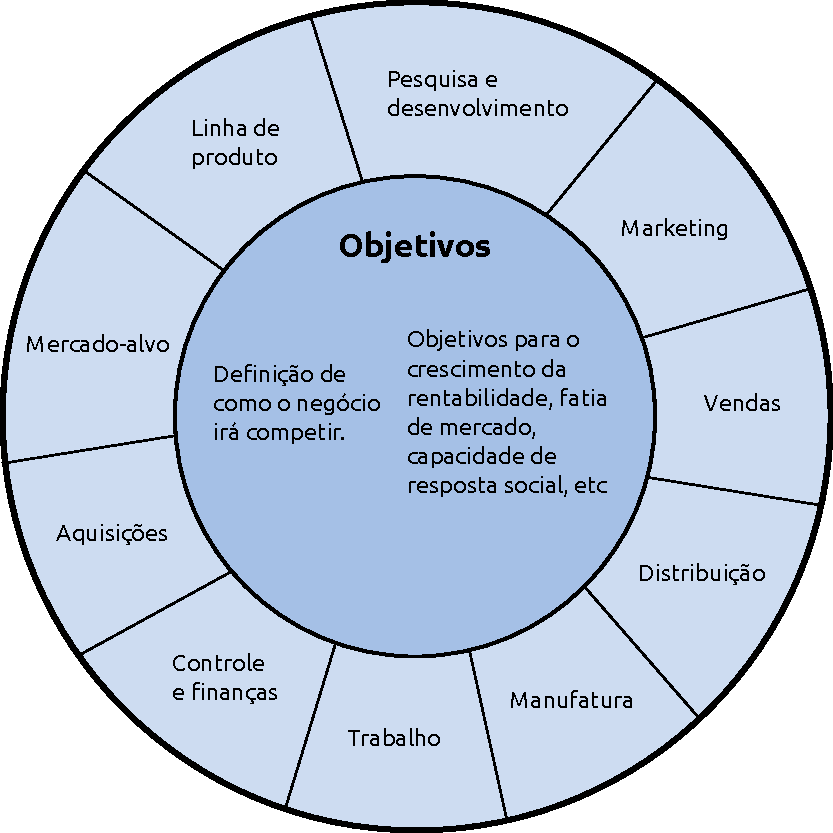
\includegraphics[scale=0.65]{../slides/imagens/estrategia.pdf}
	\end{center}
	\caption{\label{estrategia} A roda da estratégia competitiva.}
\end{figure}


